\section{Прочие резонансные процессы}

\subsection{Резонасная конверсия поляризации фотона}

Поляризационные состояния фотонов, которые обсуждались в разделе~\ref{Ch:Photon}, на практике не существуют в изолированном виде. В распространяющейся волне состояние всегда представляет собой суперпозицию этих мод.

Фотоны испытывают влияние на поляризацию двух независимых факторов: взаимодействия с виртуальными электрон-позитронными парами, чей вклад пропорционален $B^2$, и рассеяния на реальных электронах плазмы, вклад которого пропорицонален их концентрации. В некоторой точке пространства, называемой резонансной, в магнитаре плотность среды принимает такое значение, что полевой и плазменный вклады полностью компенсируют друг друга. В этой точке фотон моды 1 будет переходить в моду 2 (и наоборот). Процесс обсуждается с начала 2000-ых годов, в работе~\cite{Lai2002} была показана аналогия между конверсией поляризации фотона и эффекта Михеева-Смирнова-Вольфенштейна по переходу нейтрино между ароматами, в последовавших далее статьях~\cite{ Ho2003, vanAdelsberg2006} показана роль процесса в формировании спектра излучения магнитаров. В недавнем исследовании~\cite{Wada2025} рассмотрена трехкомпонентная плазма (ионы, электроны и позитроны), что позволяет учесть изменение спектра во время гигантских вспышек магнитаров.

Поскольку плотность среды в магнитарах меняется достаточно плавно, процесс происходит адаиабатически, и со стопроцентной вероятностью фотоны меняют свою поляризацию на противоположную. Такие резонансные точки играют важную роль в формировании поляризованного излучения магнитаров.



\subsection{Резонансное рождение аксионоподобных частиц}

И, наконец, обзор резонансных процессов был бы неполным без упоминания об 
аксионах (и ALP -- аксионоподобных частицах), 
гипотетических частицах, предложенных Печчеи и Куинн~\cite{Quinn:1977} для 
решения проблемы сохранения CP инвариантности сильных взаимодействий, 
являющихся, кроме того, наиболее вероятными кандидатами на роль холодной темной 
материи Вселенной. Их подробное обсуждение выходит далеко за рамки выбранной 
здесь темы (однако интересующийся читатель легко найдет качественные обзоры, 
например,~\cite{Kim:2010, Marsh:2016}), тем не менее мы коснемся некоторых 
работ, в которых исследовалось влияние резонанса на процессы с участием 
аксионов.

Поскольку масштаб нарушения симметрии Печчеи-Куинн, $f_a$, оказывается велик, аксионы очень слабо взаимодействуют с веществом (константа взаимодействия $f_a^{-1} \lesssim 10^{-8}$\, ГэВ$^{-1}$~\cite{Raffelt:1996}). В этой связи возникают определенные трудности на пути экспериментального обнаружения аксиона. Как уже неоднократно отмечалось ранее, влияние внешней активной среды на реакции с участием элементарных частиц и, в частности,  аксионов, в зависимости от значений параметров среды (температуры  $T$, химического потенциала  $\mu$ или индукции магнитного поля  $B$), может как катализировать эти реакции, так и оказывать дополнительное (к $f_a^{-1}$) их подавление.

Поляризованные фотоны могут вступать в реакции с псевдоскалярными частицами, такими как аксионы~\cite{Sikivie:1983}. В результате возможен такой процесс, как конверсия аксион-фотон~\cite{Raffelt:1988}, аналогичный эффекту Михеева-Смирнова-Вольфенштейна и конверсии поляризации фотона. Это взаимодействие в замагниченной плазме может быть резонансно усиленно двумя механизмами: присутствием замагниченной плазмы и четырехфотонным взаимодействием Эйлера-Гейзенбрега, который становится существенным в пределе малых энергий~\cite{Lai:2006}. Первый резонанс наблюдается в случае, когда плазменная частота приблизительно равна массе аксиона, $\omega_{pl}\simeq m_a$~\cite{Yanagida:1988}. Он может приводить к радиоизлучению, когда поток аксионов падает на нейтронную звезду~\cite{Pshirkov:2009}. Если в рамках первого механизма резонанс может наблюдаться как для релятивистских, так и для нерелятивистских аксионов, то резонанс, связанный с четырехфотонным взаимодействием, реализуется только для релятивистских аксионов.

С другой стороны, резонанс на виртуальном фотоне в реакциях общего вида $i \to f + a$, где в начальном ($i$) и конечном ($f$) состояниях могут присутствовать заряженные компоненты среды, исследовался в достаточно ограниченном списке работ~\cite{Skobelev:2000,Skobelev:2007,MikhRumShk:09}. Среди основных механизмов рождения аксиона можно выделить комптоноподобный процесс $\gamma e \to e a$~\cite{Skobelev:2000}, в котором аксион связывается с электронами и участвует в рождении фотона или в магнитотормозном излучении. Другим основным механизмом является также эффект Примакова~\cite{Primakoff:1951} -- аксион вступает во взаимодействие с виртуальным фотоном и рождает реальный. Оба процесса вместе исследовались, например, в работе~\cite{Raffelt:1996} с учетом экранирования зарядов в плазме.

В работе~\cite{Buschmann:2021} было показано, что жесткое рентгеновское 
излучение в диапазоне $2-8$ кэВ от близлежащих нейтронных звезд, которое не 
удалось связать с другими процессами, может быть объяснено следующим 
механизмом: аксионы рождаются термически внутри ядра нейтронной звезды, 
вследствие того, что они слабо взаимодействуют с веществом, они покидают звезду 
и далее превращаются в рентгеновское излучение в магнитном поле звезды.

%
\begin{figure}
\centerline{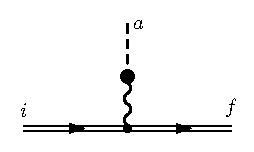
\includegraphics[width=5cm]{fig5_1.eps}}
\caption{Диаграммы Фейнмана для процесса общего вида $i \to 
f+a$. Двойные линии означают, что влияние внешнего поля на начальное и 
конечное состояния учтено точно.}
\label{fig:Diagaxion}
\end{figure}

\subsection{Фотонейтринный процесс}

Еще одним процессом, в котором может реализовываться резонанс на виртуальном электроне, является фоторождение пары нейтрино-антинейтрино на электроне, $e\gamma\to e\nu\bar\nu$, называемое фотонейтринным процессом. Наряду с другими реакциями, в которых нейтринная пара находится в конечном состоянии, интерес к нему вызван тем, что данный процесс может играть определяющую роль в остывании нейтронных звезд. Это связано с тем, что в нейтронных звездах замагниченная плазма прозрачна для нейтрино при значениях параметров (плотности и температуры), которые дают все существующие модели внутреннего строения.

Фотонейтринный процесс был впервые рассмотрен в работах~\cite{Ritus:1961,Chiu:1961}, в которых было 
вычислено сечение рассеяния  в нерелятивистском приближении. Нейтринная светимость, т.е. энергия, уносимая нейтринной парой из единичного объема за единицу времени, за счет него была вычислена в 
работах~\cite{Beaudet:1967,Dicus:1972,Munakata:1985,Shindler:1987,Itoh:1989,Itoh:1996,Skobelev:2000}.
 В частности, в~\cite{Itoh:1989,Itoh:1996} были получены таблицы с большим количеством данных для фотонейтринной излучательной способности и аналитические аппроксимации для них. При этом вклад реакции в процесс нейтринного остывания нейтронной звезды полагался пренебрежимо малым, как отмечают авторы обзора~\cite{Yakovlev2001}, поскольку в холодной и плотной плазме распад плазмона, $\gamma\to\nu\bar\nu$, является намного более эффективным каналом по уносу энергии за счет нейтринных пар.

На следующем этапе фотонейтринный процесс изучался с учетом влияния внешней активной среды на дисперсионные и поляризационные свойства фотона~\cite{RCh:2008,Borisov:2012,RumChMik}. Хотя в этих работах были получены уточнения к нейтринной светимости процесса, общий вывод о том, что фотонейтринный процесс является поправкой более высокого порядка к распаду плазмона, остался неизменным.

Наконец, в~\cite{Chistyakov:2014cga,qfthep2017} был рассмотрен резонанс в фотонейтринном процессе. Как было показано в этих работах, даже в магнитарных полях условие~(\ref{bigB}), при котором магнитное поле является доминирующим параметром среды, перестает выполняться при высоких значениях плотности плазмы $\rho \gtrsim 10^8$ г/см$^3$. Такая плотность может достигаться в границе между внешней и внутренней корой магнитара. В результате у электронов (позитронов) плазмы начинают возбуждаться высшие уровни Ландау, что приводит к возможности резонанса в этой реакции. Это может увеличивать нейтринную светимость (количество энергии, уносимое нейтринными парами из единицы объема вещества за единицу времени) за счет фотонейтринного процесса в 2-4 раза, чего, однако, недостаточно для того, чтобы он мог конкурировать по эффективности с распадом плазмона.